\documentclass[11pt,a4paper]{article}
\usepackage{amsmath, amssymb, graphicx, xcolor}

\setlength{\textwidth}{6.8in}
\setlength{\textheight}{9.6in}
\setlength{\oddsidemargin}{-0.15in}
\setlength{\evensidemargin}{-0.15in}
\setlength{\topmargin}{-0.6in}
\setlength{\headheight}{0in}
\setlength{\headsep}{0in}
\setlength{\parindent}{0pt}
\setlength{\parskip}{5pt}

\definecolor{primary}{RGB}{15, 45, 95}
\definecolor{secondary}{RGB}{30, 80, 150}
\definecolor{accent}{RGB}{180, 40, 40}
\definecolor{qboxbg}{RGB}{245, 248, 252}

\newcommand{\questionheader}[3]{
    \vspace{0.35cm}
    \noindent\colorbox{qboxbg}{
        \parbox{\dimexpr\textwidth-2\fboxsep\relax}{
            \textbf{\textcolor{primary}{\large #1}} \hfill \textbf{\textcolor{accent}{[#2]}} \hfill \textbf{\textcolor{secondary}{#3 Marks}}
        }
    }
    \vspace{0.15cm}
}

\newcommand{\sectionbanner}[1]{
    \vspace{0.5cm}
    \noindent\colorbox{primary}{
        \parbox{\dimexpr\textwidth-2\fboxsep\relax}{
            \centering \textbf{\textcolor{white}{\Large #1}}
        }
    }
    \vspace{0.25cm}
}

\begin{document}

\begin{center}
    {\LARGE \textbf{\textcolor{primary}{BRAC UNIVERSITY}}}\\[4pt]
    {\large \textbf{Department of Computer Science and Engineering}}\\[3pt]
    {\textbf{CSE421 / EEE465: Computer Networks --- Final Examination}}\\[2pt]
    \textbf{Semester:} Spring 2024 \quad | \quad \textbf{Set:} B (v2) \quad | \quad \textbf{Full Marks:} 70 \quad | \quad \textbf{Duration:} 2 Hours 5 Minutes\\[2pt]
    \rule{\textwidth}{1.5pt}
    {\large \textbf{\textcolor{secondary}{COMPREHENSIVE SOLUTION AND COMPLETE ANSWER KEY}}}
    \rule{\textwidth}{0.8pt}
\end{center}

\sectionbanner{SECTION A: MANDATORY QUESTIONS (40 MARKS)}

% =========================================================================
% QUESTION 1
% =========================================================================
\questionheader{Question 1: Hierarchical VLSM Subnetting}{CO3}{3 + 12 = 15}

\textbf{Problem Statement:}
Mahalabia Inc. needs to subnet the existing network (\texttt{1.2.128.0/17}) into smaller sub-networks as given in the topology below.

\begin{center}
    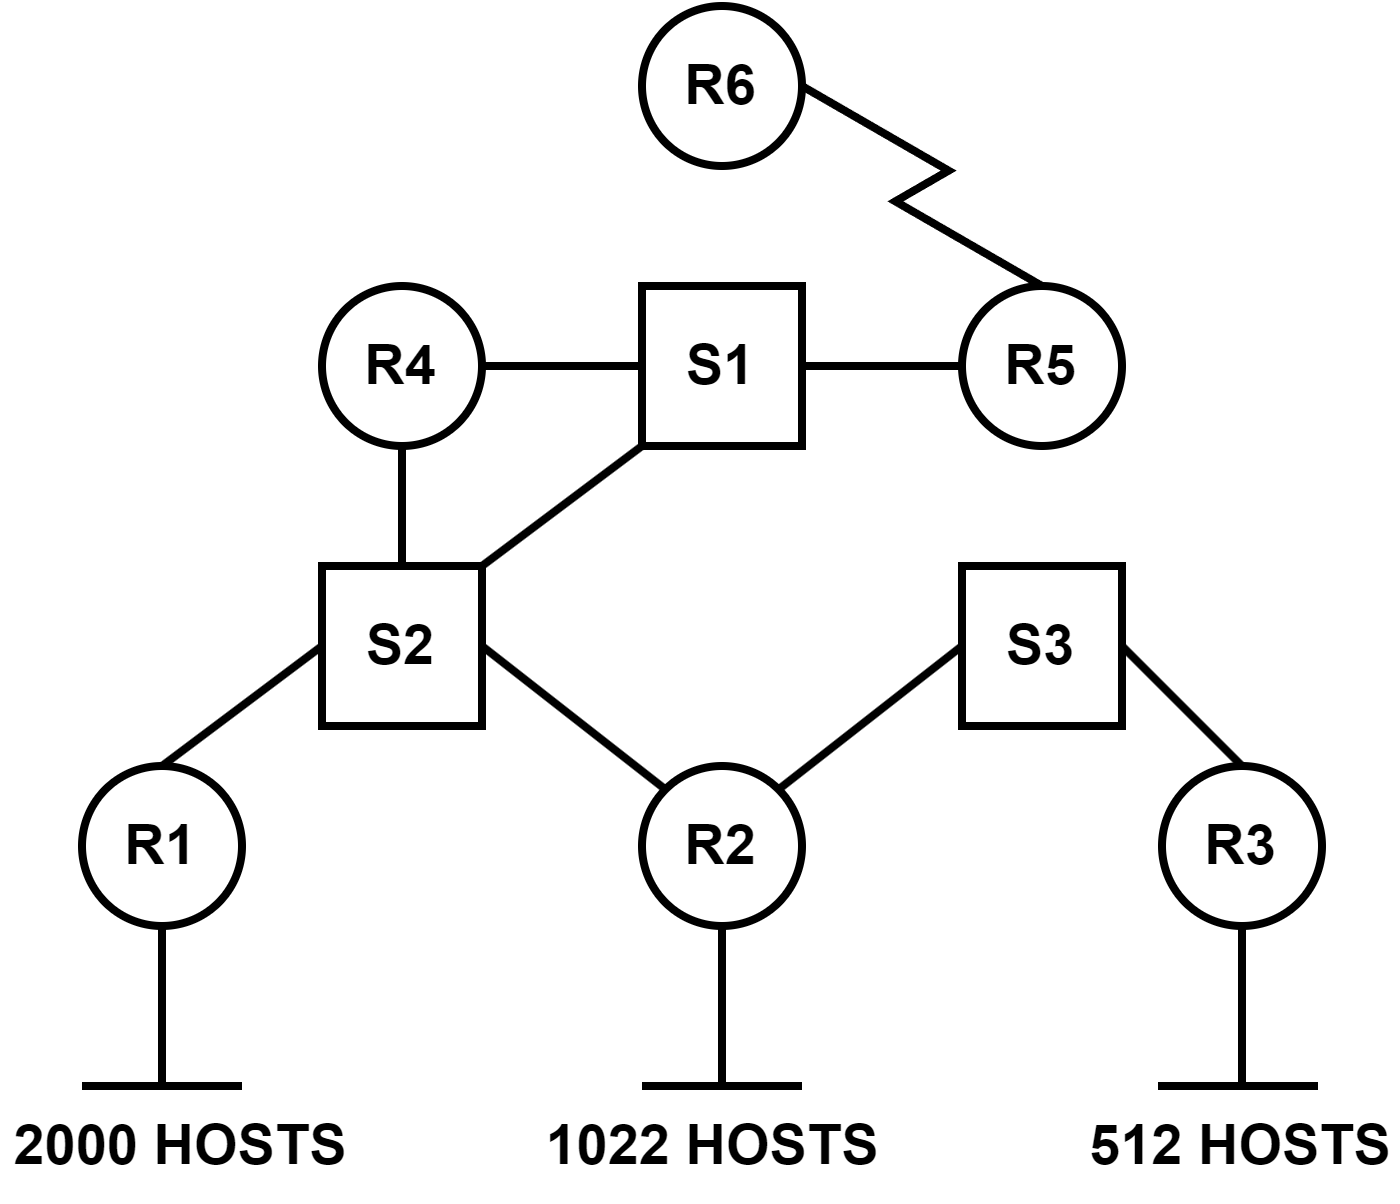
\includegraphics[width=0.45\textwidth]{p3_q1_topology.png}
\end{center}

\textbf{I. Determine the maximum number of subnets you can create from the above-mentioned root network. [3 Marks]}

\textbf{Solution:}
\begin{itemize}
    \item The root network is \texttt{1.2.128.0/17}.
    \item Total host bits available in the root network $= 32 - 17 = 15$ bits.
    \item In IPv4 network design, the smallest standard subnet capable of supporting usable host devices (such as point-to-point router WAN links) is a \textbf{$/30$} subnet (providing 2 usable host IPs, 1 network address, and 1 broadcast address).
    \item Subnet bits borrowed to create $/30$ subnets $= 30 - 17 = 13$ bits.
    \item Maximum number of $/30$ subnets:
    \[
    \text{Max Subnets} = 2^{13} = \mathbf{8192\text{ subnets}}
    \]
    \textit{(Note: If considering theoretical host routes of prefix $/32$, $2^{32-17} = 2^{15} = 32,768$ individual addresses)}.
\end{itemize}
\textbf{Answer:} \textbf{8,192 subnets} (at $/30$).

\vspace{0.2cm}
\textbf{II. Efficiently calculate the network address for all the sub-networks and draw the hierarchical tree. [12 Marks]}

\textbf{0.1 Topology Requirement Analysis \& Subnet Identification:}
In IPv4 network architecture, subnets (broadcast domains) are demarcated by router Layer 3 interfaces. Analyzing the given multi-router campus topology:
\begin{itemize}
    \item \textbf{LAN Subnets (End Devices):}
    \begin{enumerate}
        \item \textbf{R1 LAN:} Requires \textbf{2000 Hosts}.
        \item \textbf{R2 LAN:} Requires \textbf{1022 Hosts}.
        \item \textbf{R3 LAN:} Requires \textbf{512 Hosts}.
    \end{enumerate}
    \item \textbf{Inter-Router Subnets (Switches \& WAN Links):}
    \begin{enumerate}
        \setcounter{enumi}{3}
        \item \textbf{Switch S2 Subnet:} Connects router interfaces of \textbf{R1, R2, and R4} $\implies$ \textbf{3 Hosts} (3 router IP interfaces).
        \item \textbf{Switch S1 Subnet:} Connects router interfaces of \textbf{R4 and R5} $\implies$ \textbf{2 Hosts} (2 router IP interfaces).
        \item \textbf{Switch S3 Subnet:} Connects router interfaces of \textbf{R2 and R3} $\implies$ \textbf{2 Hosts} (2 router IP interfaces).
        \item \textbf{WAN Link (R5--R6):} Point-to-point serial link between \textbf{R5 and R6} $\implies$ \textbf{2 Hosts} (2 router IP interfaces).
    \end{enumerate}
    \textit{(Architectural Note: If the diagonal inter-switch link between S1 and S2 is treated as a unified Layer 2 broadcast domain, S1 and S2 would merge into a single transit subnet connecting 4 router interfaces R1, R2, R4, R5 requiring $H=4 \implies /29$. Operating S1 and S2 as distinct routed subnets provides 7 dedicated, cleanly separated subnets as derived below).}
\end{itemize}

\vspace{0.2cm}
\textbf{0.2 Step-by-Step Derivations (Following the 6-Step Method):}

\textbf{1. Subnet 1: R1 LAN (2000 Hosts --- Largest)}
\begin{itemize}
    \item \textbf{Step 1 (Capacity $H_2$):} $H_2 = H + 2 = 2000 + 2 = 2002$
    \item \textbf{Step 2 (Host Bits $H_b$):} $H_b = \lceil \log_2(2002) \rceil = 11\text{ bits}$ ($2^{10} = 1024 < 2002 \le 2^{11} = 2048$)
    \item \textbf{Step 3 (Prefix $P$):} $P = 32 - 11 = \mathbf{/21}$
    \item \textbf{Step 4 (Allocated IPs):} $2^{11} = 2048\text{ IPs}$ (Block size in 3rd octet $= 2048 / 256 = 8$)
    \item \textbf{Step 5 (Addresses):}
    \begin{itemize}
        \item Network Address: \texttt{1.2.128.0/21}
        \item Usable Host Range: \texttt{1.2.128.1} to \texttt{1.2.135.254}
        \item Directed Broadcast Address: \texttt{1.2.135.255}
        \item Next Subnet Base IP: \texttt{1.2.(128 + 8).0} = \texttt{1.2.136.0}
    \end{itemize}
    \item \textbf{Step 6 (Subnet Mask):} $255.255.(256 - 8).0 = \mathbf{255.255.248.0}$
\end{itemize}

\textbf{2. Subnet 2: R2 LAN (1022 Hosts)}
\begin{itemize}
    \item \textbf{Step 1 (Capacity $H_2$):} $H_2 = H + 2 = 1022 + 2 = 1024$
    \item \textbf{Step 2 (Host Bits $H_b$):} $H_b = \lceil \log_2(1024) \rceil = 10\text{ bits}$ ($2^9 = 512 < 1024 \le 2^{10} = 1024$)
    \item \textbf{Step 3 (Prefix $P$):} $P = 32 - 10 = \mathbf{/22}$
    \item \textbf{Step 4 (Allocated IPs):} $2^{10} = 1024\text{ IPs}$ (Block size in 3rd octet $= 1024 / 256 = 4$)
    \item \textbf{Step 5 (Addresses):}
    \begin{itemize}
        \item Network Address: \texttt{1.2.136.0/22}
        \item Usable Host Range: \texttt{1.2.136.1} to \texttt{1.2.139.254}
        \item Directed Broadcast Address: \texttt{1.2.139.255}
        \item Next Subnet Base IP: \texttt{1.2.(136 + 4).0} = \texttt{1.2.140.0}
    \end{itemize}
    \item \textbf{Step 6 (Subnet Mask):} $255.255.(256 - 4).0 = \mathbf{255.255.252.0}$
\end{itemize}

\textbf{3. Subnet 3: R3 LAN (512 Hosts)}
\begin{itemize}
    \item \textbf{Step 1 (Capacity $H_2$):} $H_2 = H + 2 = 512 + 2 = 514$
    \item \textbf{Step 2 (Host Bits $H_b$):} $H_b = \lceil \log_2(514) \rceil = 10\text{ bits}$ ($2^9 = 512 < 514 \le 2^{10} = 1024$)
    \item \textbf{Step 3 (Prefix $P$):} $P = 32 - 10 = \mathbf{/22}$
    \item \textbf{Step 4 (Allocated IPs):} $2^{10} = 1024\text{ IPs}$ (Block size in 3rd octet $= 4$)
    \item \textbf{Step 5 (Addresses):}
    \begin{itemize}
        \item Network Address: \texttt{1.2.140.0/22}
        \item Usable Host Range: \texttt{1.2.140.1} to \texttt{1.2.143.254}
        \item Directed Broadcast Address: \texttt{1.2.143.255}
        \item Next Subnet Base IP: \texttt{1.2.(140 + 4).0} = \texttt{1.2.144.0}
    \end{itemize}
    \item \textbf{Step 6 (Subnet Mask):} $255.255.(256 - 4).0 = \mathbf{255.255.252.0}$
    \item \textit{(Alternative Note: If 512 was loosely intended as the power-of-two block allocation $2^9$, then $H_b = 9 \implies /23$ with 510 usable hosts, spanning \texttt{1.2.140.0/23} and freeing \texttt{1.2.142.0} for subsequent subnets)}.
\end{itemize}

\textbf{4. Subnet 4: Switch S2 Subnet (3 Hosts: R1, R2, R4)}
\begin{itemize}
    \item \textbf{Step 1 (Capacity $H_2$):} $H_2 = 3 + 2 = 5$
    \item \textbf{Step 2 (Host Bits $H_b$):} $H_b = \lceil \log_2(5) \rceil = 3\text{ bits}$ ($2^2 = 4 < 5 \le 2^3 = 8$)
    \item \textbf{Step 3 (Prefix $P$):} $P = 32 - 3 = \mathbf{/29}$
    \item \textbf{Step 4 (Allocated IPs):} $2^3 = 8\text{ IPs}$
    \item \textbf{Step 5 (Addresses):}
    \begin{itemize}
        \item Network Address: \texttt{1.2.144.0/29}
        \item Usable Host Range: \texttt{1.2.144.1} to \texttt{1.2.144.6}
        \item Directed Broadcast Address: \texttt{1.2.144.7}
        \item Next Subnet Base IP: \texttt{1.2.144.0 + 8} = \texttt{1.2.144.8}
    \end{itemize}
    \item \textbf{Step 6 (Subnet Mask):} $255.255.255.(256 - 8) = \mathbf{255.255.255.248}$
\end{itemize}

\textbf{5. Subnet 5: Switch S1 Subnet (2 Hosts: R4, R5)}
\begin{itemize}
    \item \textbf{Step 1 (Capacity $H_2$):} $H_2 = 2 + 2 = 4$
    \item \textbf{Step 2 (Host Bits $H_b$):} $H_b = \lceil \log_2(4) \rceil = 2\text{ bits}$ ($2^2 = 4$)
    \item \textbf{Step 3 (Prefix $P$):} $P = 32 - 2 = \mathbf{/30}$
    \item \textbf{Step 4 (Allocated IPs):} $2^2 = 4\text{ IPs}$
    \item \textbf{Step 5 (Addresses):}
    \begin{itemize}
        \item Network Address: \texttt{1.2.144.8/30}
        \item Usable Host Range: \texttt{1.2.144.9} to \texttt{1.2.144.10}
        \item Directed Broadcast Address: \texttt{1.2.144.11}
        \item Next Subnet Base IP: \texttt{1.2.144.8 + 4} = \texttt{1.2.144.12}
    \end{itemize}
    \item \textbf{Step 6 (Subnet Mask):} $255.255.255.(256 - 4) = \mathbf{255.255.255.252}$
\end{itemize}

\textbf{6. Subnet 6: Switch S3 Subnet (2 Hosts: R2, R3)}
\begin{itemize}
    \item \textbf{Step 1 (Capacity $H_2$):} $H_2 = 2 + 2 = 4 \implies H_b = 2\text{ bits}$
    \item \textbf{Step 3 (Prefix $P$):} $P = 32 - 2 = \mathbf{/30}$, Total Allocated IPs = 4
    \item \textbf{Step 5 (Addresses):}
    \begin{itemize}
        \item Network Address: \texttt{1.2.144.12/30}
        \item Usable Host Range: \texttt{1.2.144.13} to \texttt{1.2.144.14}
        \item Directed Broadcast Address: \texttt{1.2.144.15}
        \item Next Subnet Base IP: \texttt{1.2.144.12 + 4} = \texttt{1.2.144.16}
    \end{itemize}
    \item \textbf{Step 6 (Subnet Mask):} $\mathbf{255.255.255.252}$
\end{itemize}

\textbf{7. Subnet 7: WAN Serial Link R5--R6 (2 Hosts)}
\begin{itemize}
    \item \textbf{Step 1 (Capacity $H_2$):} $H_2 = 2 + 2 = 4 \implies H_b = 2\text{ bits}$
    \item \textbf{Step 3 (Prefix $P$):} $P = 32 - 2 = \mathbf{/30}$, Total Allocated IPs = 4
    \item \textbf{Step 5 (Addresses):}
    \begin{itemize}
        \item Network Address: \texttt{1.2.144.16/30}
        \item Usable Host Range: \texttt{1.2.144.17} to \texttt{1.2.144.18}
        \item Directed Broadcast Address: \texttt{1.2.144.19}
        \item Next Available Base IP: \texttt{1.2.144.20}
    \end{itemize}
    \item \textbf{Step 6 (Subnet Mask):} $\mathbf{255.255.255.252}$
\end{itemize}

\vspace{0.3cm}
\textbf{0.3 Complete Master VLSM Allocation Table:}

\begin{center}
\small
\setlength{\tabcolsep}{3.5pt}
\begin{tabular}{|l|c|c|c|l|l|l|}
\hline
\textbf{Subnet Name} & \textbf{Req. Hosts ($H$)} & \textbf{$H_b$} & \textbf{Prefix} & \textbf{Network IP} & \textbf{Usable Host Range} & \textbf{Subnet Mask} \\
\hline
\textbf{R1 LAN} & 2000 & 11 & /21 & \texttt{1.2.128.0} & \texttt{1.2.128.1} -- \texttt{1.2.135.254} & \texttt{255.255.248.0} \\
\textbf{R2 LAN} & 1022 & 10 & /22 & \texttt{1.2.136.0} & \texttt{1.2.136.1} -- \texttt{1.2.139.254} & \texttt{255.255.252.0} \\
\textbf{R3 LAN} & 512  & 10 & /22 & \texttt{1.2.140.0} & \texttt{1.2.140.1} -- \texttt{1.2.143.254} & \texttt{255.255.252.0} \\
\textbf{Switch S2 (R1, R2, R4)} & 3 & 3 & /29 & \texttt{1.2.144.0} & \texttt{1.2.144.1} -- \texttt{1.2.144.6} & \texttt{255.255.255.248} \\
\textbf{Switch S1 (R4, R5)}     & 2 & 2 & /30 & \texttt{1.2.144.8} & \texttt{1.2.144.9} -- \texttt{1.2.144.10} & \texttt{255.255.255.252} \\
\textbf{Switch S3 (R2, R3)}     & 2 & 2 & /30 & \texttt{1.2.144.12} & \texttt{1.2.144.13} -- \texttt{1.2.144.14} & \texttt{255.255.255.252} \\
\textbf{WAN Link (R5--R6)}      & 2 & 2 & /30 & \texttt{1.2.144.16} & \texttt{1.2.144.17} -- \texttt{1.2.144.18} & \texttt{255.255.255.252} \\
\hline
\end{tabular}
\end{center}

\vspace{0.2cm}
\textbf{0.4 Hierarchical Subnet Tree:}
\begin{verbatim}
1.2.128.0/17 (Root Network, 32,768 IPs: 1.2.128.0 to 1.2.255.255)
 |-- 1.2.128.0/18 (First Branch: 16,384 IPs: 1.2.128.0 to 1.2.191.255)
 |    |-- 1.2.128.0/21  [R1 LAN: 2000 Hosts] (2,048 IPs)
 |    |-- 1.2.136.0/22  [R2 LAN: 1022 Hosts] (1,024 IPs)
 |    |-- 1.2.140.0/22  [R3 LAN: 512 Hosts]  (1,024 IPs)
 |    `-- 1.2.144.0/22  (Transit & Core Blocks)
 |         |-- 1.2.144.0/29   [Switch S2: R1, R2, R4] (8 IPs)
 |         |-- 1.2.144.8/30   [Switch S1: R4, R5]     (4 IPs)
 |         |-- 1.2.144.12/30  [Switch S3: R2, R3]     (4 IPs)
 |         |-- 1.2.144.16/30  [WAN Link: R5--R6]      (4 IPs)
 |         `-- 1.2.144.20/30 ... 1.2.147.255 (Free Unallocated Pool)
 `-- 1.2.192.0/18 (Second Branch: 16,384 IPs Reserved for Future Campus Expansion)
\end{verbatim}

\newpage
% =========================================================================
% QUESTION 2
% =========================================================================
\questionheader{Question 2: Route Summarization \& Floating Static Route}{CO3}{6 + 4 = 10}

\begin{center}
    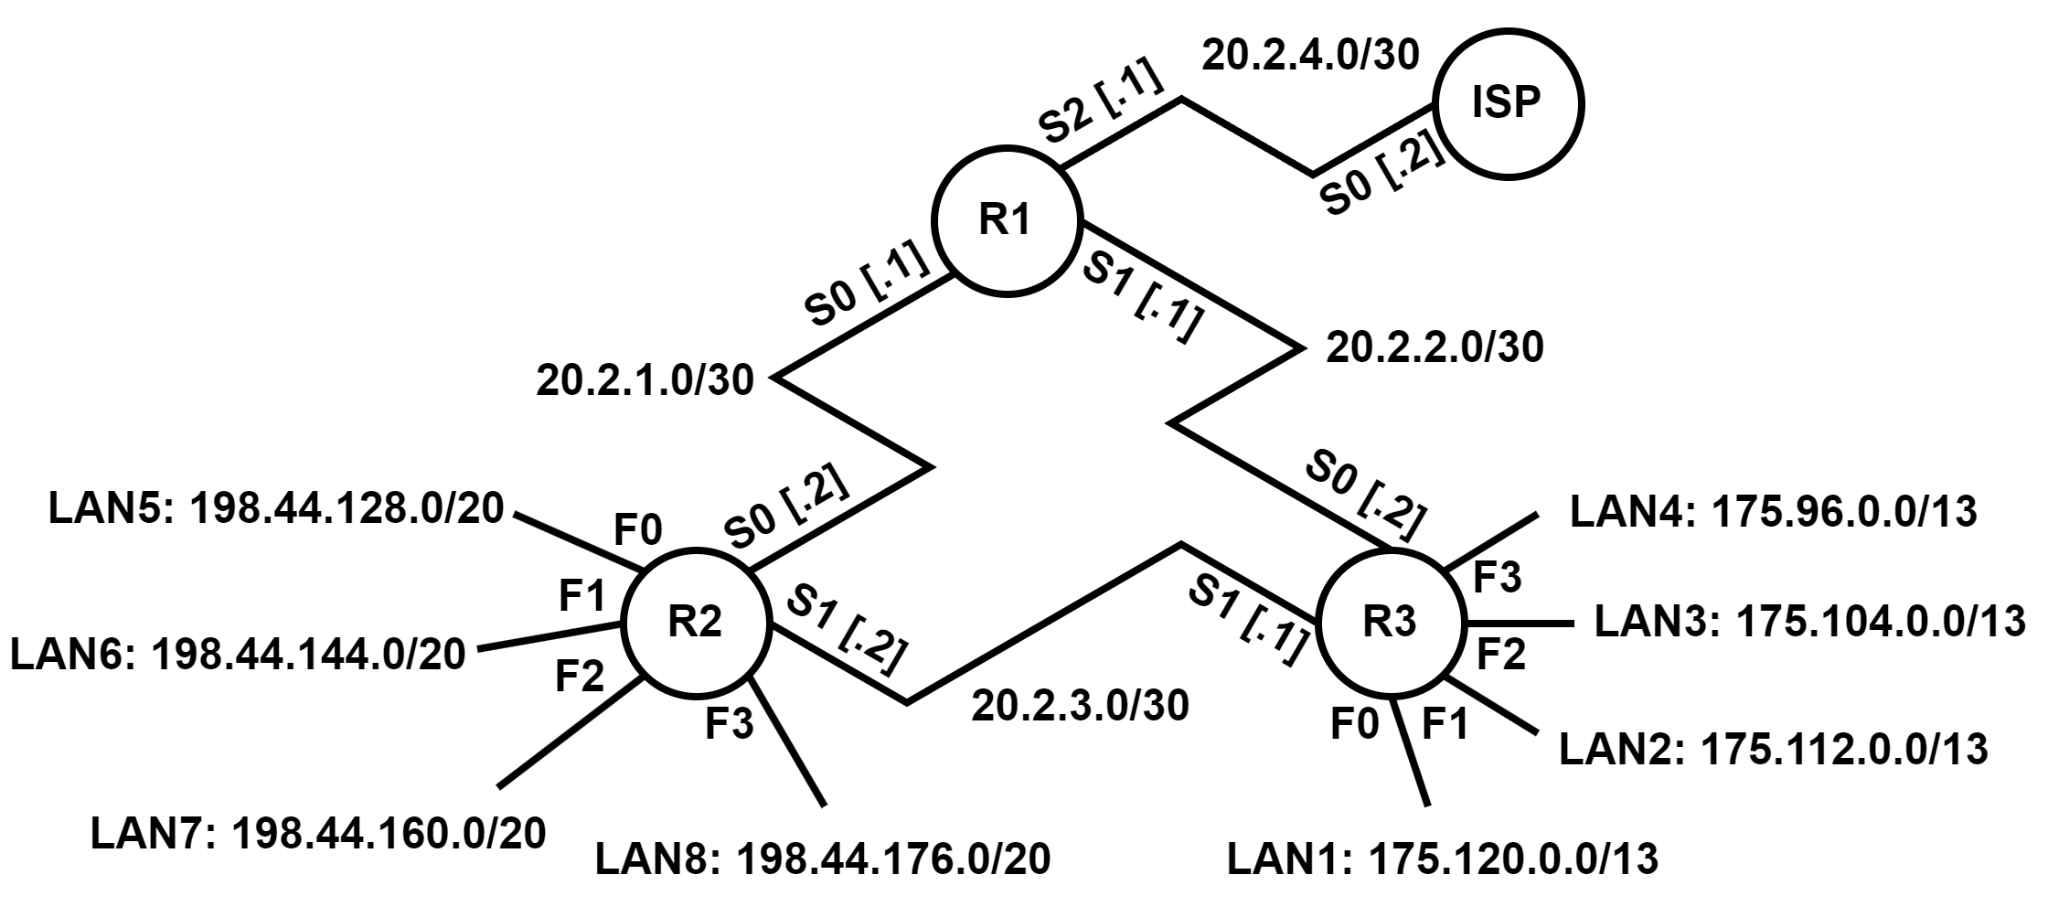
\includegraphics[width=0.7\textwidth]{p3_q2_topology.png}
\end{center}

\textbf{I. Calculate the summarized network of all R3 LANs and configure a summary static route in R1. [6 Marks]}

\textbf{Solution:}
\begin{enumerate}
    \item \textbf{List R3 LANs:}
    \begin{itemize}
        \item LAN4: \texttt{175.96.0.0/13}
        \item LAN3: \texttt{175.104.0.0/13}
        \item LAN2: \texttt{175.112.0.0/13}
        \item LAN1: \texttt{175.120.0.0/13}
    \end{itemize}

    \item \textbf{Binary Expansion of Second Octet:}
    \[
    \begin{aligned}
    96_{10}  &= \mathbf{011}00000_2 \\
    104_{10} &= \mathbf{011}01000_2 \\
    112_{10} &= \mathbf{011}10000_2 \\
    120_{10} &= \mathbf{011}11000_2
    \end{aligned}
    \]
    The first 3 bits of the second octet (\texttt{011}) are identical across all four networks.
    \item Total common network bits $= 8 \text{ (1st octet)} + 3 \text{ (2nd octet)} = \mathbf{/11}$.
    \item Summarized Network Address: \textbf{\texttt{175.96.0.0/11}}
    \item Subnet Mask for $/11$: \textbf{\texttt{255.224.0.0}}
    \item \textbf{Configuration Command on Router R1:}
    R1 reaches R3 directly via interface \texttt{S1} (link \texttt{20.2.2.0/30}, R3 is \texttt{S0 [.2]} $\to$ next-hop IP \texttt{20.2.2.2}):
    \begin{center}
        \texttt{R1(config)\# ip route 175.96.0.0 255.224.0.0 20.2.2.2}
    \end{center}
    \textit{(or specifying exit interface: \texttt{R1(config)\# ip route 175.96.0.0 255.224.0.0 S1})}.
\end{enumerate}

\vspace{0.2cm}
\textbf{II. Floating Static Route on R1 to LAN2 of R3 via R2 with AD = 50. [4 Marks]}

\textbf{Solution:}
\begin{itemize}
    \item Destination Network: LAN2 of R3 = \texttt{175.112.0.0/13} (Subnet Mask: \texttt{255.248.0.0}).
    \item Outbound exit interface towards Router R2 is \textbf{\texttt{S0}} (link \texttt{20.2.1.0/30}).
    \item Next-hop IP on Router R2 is \texttt{20.2.1.2}.
    \item Administrative Distance required: \textbf{50}.
    \item Cisco IOS Command on R1:
    \begin{center}
        \texttt{R1(config)\# ip route 175.112.0.0 255.248.0.0 S0 50}
    \end{center}
    \textit{(or with next-hop IP: \texttt{R1(config)\# ip route 175.112.0.0 255.248.0.0 S0 20.2.1.2 50})}.
\end{itemize}

% =========================================================================
% QUESTION 3
% =========================================================================
\questionheader{Question 3: IPv4 Fragmentation Analysis}{CO3}{2 + 2 + 1 = 5}

\textbf{Given:}
\begin{itemize}
    \item Original datagram total length $= 4560$ bytes (includes 20-byte IP header).
    \item Outbound serial link MTU $= 380$ bytes.
\end{itemize}

\textbf{I. Calculate the number of fragments created. [2 Marks]}
\begin{itemize}
    \item Total original payload data $= 4560 - 20 = 4540$ bytes.
    \item Maximum payload per fragment $\le 380 - 20 = 360$ bytes.
    \item Since $360 / 8 = 45$ is an exact multiple of 8, each intermediate fragment carries exactly \textbf{360 bytes of data}.
    \item Number of full 360-byte fragments $= \lfloor 4540 / 360 \rfloor = 12$ fragments.
    \item Data accounted for by first 12 fragments $= 12 \times 360 = 4320$ bytes.
    \item Remaining data for the 13th (last) fragment $= 4540 - 4320 = 220$ bytes.
    \item \textbf{Total number of fragments} $= 12 + 1 = \mathbf{13\text{ fragments}}$.
\end{itemize}

\textbf{II. Calculate the fragment offset of the 4th fragment. [2 Marks]}
\begin{itemize}
    \item Using the standard fragment offset formula from the networking study notes:
    \[
    \text{Fragment Offset}_k = \frac{(k - 1) \times \text{Payload}}{8}
    \]
    where $k$ is the fragment index ($k = 4$) and $\text{Payload} = 360\text{ bytes}$ is the data payload per full fragment.
    \item Substituting $k = 4$ and $\text{Payload} = 360$:
    \[
    \text{Offset}_4 = \frac{(4 - 1) \times 360}{8} = \frac{3 \times 360}{8} = 3 \times 45 = \mathbf{135}
    \]
    \item (Verification: The starting byte in the original unfragmented payload is $3 \times 360 = 1080\text{ bytes}$, spanning bytes 1080 to 1439).
\end{itemize}
\textbf{Answer:} \textbf{135}.

\textbf{III. State the MF bit of the 5th fragment. [1 Mark]}
\begin{itemize}
    \item Since there are 13 fragments, the 5th fragment is an intermediate fragment ($5 < 13$).
    \item Therefore, More Fragments flag: $\mathbf{MF = 1}$.
\end{itemize}

\newpage
% =========================================================================
% QUESTION 4
% =========================================================================
\questionheader{Question 4: DHCP Cross-Router Limitation \& Relay Agent Solution}{CO2}{6}

\textbf{Problem Statement:}
Dipu tries to share Zahin's DHCP server located two floors down in another company's network. However, Dipu's devices cannot receive any IP configuration from the DHCP server. Identify the problem and explain the solution.

\textbf{Solution:}
\begin{enumerate}
    \item \textbf{Identification of the Problem [3 Marks]:}
    \begin{itemize}
        \item When Dipu's client devices boot up, they broadcast \textbf{DHCPDISCOVER} messages with destination IP \texttt{255.255.255.255} and destination MAC \texttt{FF:FF:FF:FF:FF:FF}.
        \item Zahin's DHCP server resides on a different network across one or more intermediate routers.
        \item By architectural design, \textbf{routers do not forward Layer 2 or Layer 3 broadcast frames} across broadcast domain boundaries.
        \item Therefore, the DHCPDISCOVER messages are blocked at Dipu's local router and never reach Zahin's DHCP server.
    \end{itemize}
    \item \textbf{Solution [3 Marks]:}
    \begin{itemize}
        \item Configure Dipu's router interface as a \textbf{DHCP Relay Agent} (using the Cisco IOS command \texttt{ip helper-address <Zahin\_DHCP\_Server\_IP>} on the router interface connected to Dipu's LAN).
        \item The router intercepts the broadcast DHCP packets, converts them into unicast UDP packets, sets the \texttt{giaddr} field to the router's local interface IP, and forwards them directly to Zahin's DHCP server.
        \item Zahin's DHCP server uses the \texttt{giaddr} to select the correct IP address pool for Dipu's subnet and unicasts the reply back to the router, which forwards it to Dipu's devices.
    \end{itemize}
\end{enumerate}

% =========================================================================
% QUESTION 5
% =========================================================================
\questionheader{Question 5: Single Public IP \& Port Address Translation (PAT)}{CO2}{4}

\textbf{Question:} Dipu can only afford a single public IP address. So, the ISP allows only one device to access the Internet. State if this statement is true or false, and explain your answer.

\textbf{Solution:}
\begin{itemize}
    \item \textbf{The statement is FALSE.}
    \item \textbf{Technical Explanation:}
    \begin{itemize}
        \item Even with only a single public IP address, all twenty devices in Dipu's startup company can simultaneously access the Internet using \textbf{Port Address Translation (PAT)}, also known as \textbf{NAT Overload}.
        \item PAT allows multiple private hosts (using RFC 1918 addresses like \texttt{192.168.1.0/24}) to share a single public IP address by mapping each connection to a unique Layer 4 source port number (TCP or UDP).
        \item Since there are approximately 64,512 usable dynamic port numbers per IP, the router can maintain thousands of concurrent sessions for multiple devices at the same time.
    \end{itemize}
\end{itemize}

\newpage
\sectionbanner{SECTION B: ANY TWO OUT OF THREE (12 MARKS)}
\textit{(All questions solved below for complete coverage)}

% =========================================================================
% QUESTION 6
% =========================================================================
\questionheader{Question 6: Distance Vector Periodic Routing Updates}{CO3}{6}

\textbf{Question:} Refer to the figure in Q2. Assume all routers run Distance Vector Routing. Through which interfaces will Router R2 send routing updates periodically? Explain your answer.

\textbf{Solution:}
\begin{itemize}
    \item In Distance Vector routing (e.g., RIPv2), routers periodically advertise their entire routing table out of \textbf{all active interfaces participating in the routing protocol process}.
    \item Looking at Router R2:
    \begin{itemize}
        \item Interface \texttt{S0} connects to Router R1 (WAN link \texttt{20.2.1.0/30}).
        \item Interface \texttt{S1} connects to Router R3 (WAN link \texttt{20.2.3.0/30}).
        \item Interfaces \texttt{F0, F1, F2, F3} connect to LAN5, LAN6, LAN7, and LAN8.
    \end{itemize}
    \item \textbf{Routing Adjacencies:} Router R2 must send dynamic routing updates across its serial interfaces \textbf{\texttt{S0}} (to R1) and \textbf{\texttt{S1}} (to R3) so that adjacent routers learn about R2's LANs and transit paths.
    \item On the LAN interfaces (\texttt{F0--F3}), by default RIP sends updates, but in professional network practice, these are configured as \textbf{passive interfaces} (\texttt{passive-interface}) to prevent advertising routing information onto user networks where no routers exist.
    \item Therefore, active periodic routing exchange occurs through interfaces \textbf{\texttt{S0}} and \textbf{\texttt{S1}}.
\end{itemize}

% =========================================================================
% QUESTION 7
% =========================================================================
\questionheader{Question 7: EUI-64 MAC Extraction \& IPv6 Classification}{CO3}{4 + 2 = 6}

\textbf{Given IPv6 Address:} \texttt{FE80:0:0:B0B:980:FF:FE00::}

\textbf{I. Identify the MAC address of your device. [4 Marks]}

\textbf{Solution:}
\begin{enumerate}
    \item The 128-bit IPv6 address expands to:
    \[
    \texttt{fe80:0000:0000:0b0b : 0980:00ff:fe00:0000}
    \]
    \item The lower 64 bits form the EUI-64 Interface Identifier:
    \[
    \text{Interface ID} = \texttt{0980:00ff:fe00:0000}
    \]
    \item In EUI-64 generation:
    \begin{itemize}
        \item The reserved delimiter bytes \texttt{FF:FE} were inserted between the 3rd and 4th bytes of the 48-bit MAC address.
        \item Removing \texttt{FF:FE} yields the 6 bytes: \texttt{09 : 80 : 00 : 00 : 00 : 00}.
        \item The 7th bit (Universal/Local bit) of the first byte was inverted during generation.
    \end{itemize}
    \item Reversing the 7th bit inversion on the first byte (\texttt{09}):
    \[
    09_{16} = 000010\mathbf{0}1_2 \xrightarrow{\text{Invert bit 7}} 000010\mathbf{1}1_2 = 0B_{16}
    \]
    \item Therefore, the original 48-bit MAC address is:
    \[
    \mathbf{0B:80:00:00:00:00} \quad (\text{or } \texttt{0b:80:00:00:00:00})
    \]
\end{enumerate}

\vspace{0.2cm}
\textbf{II. Identify the type of IPv6 address. [2 Marks]}
\begin{itemize}
    \item The address prefix is \texttt{FE80::/10}.
    \item \textbf{Answer:} \textbf{Link-Local Unicast Address}.
\end{itemize}

% =========================================================================
% QUESTION 8
% =========================================================================
\questionheader{Question 8: Switch Forwarding Behavior (Unicasting vs. Flooding)}{CO2}{4 + 2 = 6}

\begin{center}
    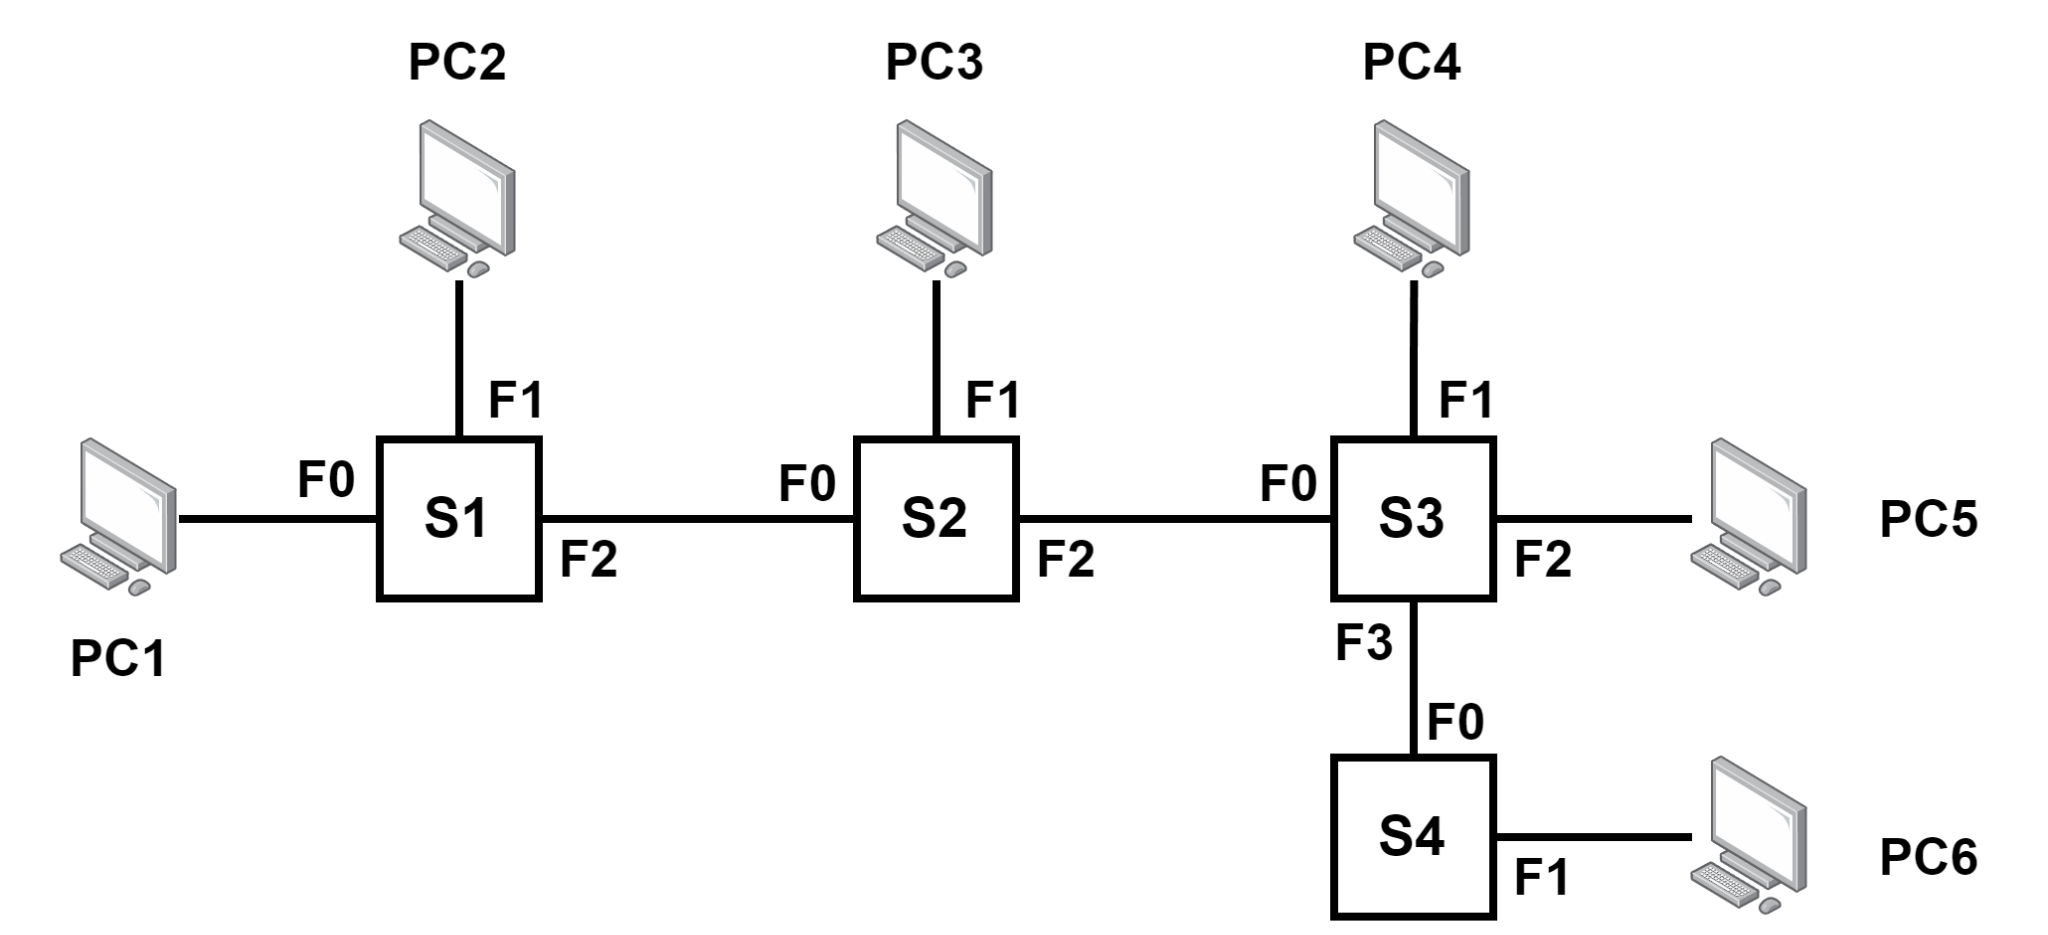
\includegraphics[width=0.7\textwidth]{p3_q8_topology.png}
\end{center}

\textbf{Initial MAC Tables:}
\begin{itemize}
    \item S2 contains: PC3 on \texttt{F1}, PC5 on \texttt{F2}.
    \item S3 contains: PC3 on \texttt{F0}, PC5 on \texttt{F2}.
    \item PC4 sends frames to PC3 and PC2. None of them replies.
\end{itemize}

\textbf{I. How sending these two frames by switch S3 is different [4 Marks]:}
\begin{enumerate}
    \item \textbf{Frame to PC3 (Known Unicast):}
    \begin{itemize}
        \item Switch S3 already has an entry for PC3 pointing to port \textbf{\texttt{F0}}.
        \item Therefore, S3 performs \textbf{selective unicasting}: it forwards the frame solely out of port \texttt{F0} towards S2.
    \end{itemize}
    \item \textbf{Frame to PC2 (Unknown Unicast):}
    \begin{itemize}
        \item S3 has no entry for PC2 in its MAC address table.
        \item Therefore, S3 performs \textbf{flooding}: it broadcasts the frame out of all active ports except the incoming port: \texttt{F0} (towards S2), \texttt{F2} (towards PC5), and \texttt{F3} (towards S4).
    \end{itemize}
\end{enumerate}

\vspace{0.2cm}
\textbf{II. Current state of MAC tables of S3 and S2 [2 Marks]:}
\begin{itemize}
    \item When PC4 transmits, S3 receives the frame on port \textbf{\texttt{F1}} and learns: \textbf{PC4 $\to$ \texttt{F1}}.
    \item The frame exits S3 on \texttt{F0} and enters S2 on port \textbf{\texttt{F2}}. S2 learns: \textbf{PC4 $\to$ \texttt{F2}}.
\end{itemize}

\begin{center}
\begin{tabular}{|l|c|}
\multicolumn{2}{c}{\textbf{Switch S3 MAC Table}} \\
\hline
\textbf{Device / MAC} & \textbf{Port} \\
\hline
PC3 & \texttt{F0} \\
PC5 & \texttt{F2} \\
\textbf{PC4} & \textbf{\texttt{F1}} \\
\hline
\end{tabular}
\qquad
\begin{tabular}{|l|c|}
\multicolumn{2}{c}{\textbf{Switch S2 MAC Table}} \\
\hline
\textbf{Device / MAC} & \textbf{Port} \\
\hline
PC3 & \texttt{F1} \\
PC5 & \texttt{F2} \\
\textbf{PC4} & \textbf{\texttt{F2}} \\
\hline
\end{tabular}
\end{center}

\newpage
\sectionbanner{SECTION C: ANY THREE OUT OF FIVE (18 MARKS)}
\textit{(All questions solved below for complete coverage)}

% =========================================================================
% QUESTION 9
% =========================================================================
\questionheader{Question 9: Denial-of-Service via Ping (ICMP Flood / Smurf)}{CO2}{2 + 4 = 6}

\textbf{I. Name of the Attack [2 Marks]:}
\textbf{ICMP Flood Attack} (or \textbf{Smurf Attack} / \textbf{Ping Flood DoS}).

\textbf{II. Process Explanation [4 Marks]:}
\begin{itemize}
    \item In an \textbf{ICMP Flood}, the attacker (or a distributed botnet) overwhelms the target web server by sending an enormous flood of ICMP Echo Request packets faster than the server can handle.
    \item In a \textbf{Smurf Attack}, the attacker broadcasts ICMP Echo Requests with the source address spoofed as the victim's web server IP to an amplification network. Hundreds of devices simultaneously send ICMP Echo Replies back to the victim.
    \item The victim's network bandwidth becomes saturated, and its operating system CPU/memory resources are consumed responding to ICMP traffic, rendering the server completely unresponsive to legitimate incoming HTTP requests.
\end{itemize}

% =========================================================================
% QUESTION 10
% =========================================================================
\questionheader{Question 10: ARP Request Forwarding \& Host Next Steps}{CO2}{2 + 4 = 6}

\textbf{Context:} Using the figure in Q8, PC1 sends an ARP request for PC5's MAC address.

\textbf{I. How switches S1, S2, S3 forward this request [2 Marks]:}
\begin{itemize}
    \item An ARP Request is a broadcast frame (Destination MAC: \texttt{FF:FF:FF:FF:FF:FF}).
    \item \textbf{S1:} Receives frame on \texttt{F0}, learns PC1 on \texttt{F0}, and \textbf{floods} it out of \texttt{F1} (to PC2) and \texttt{F2} (to S2).
    \item \textbf{S2:} Receives frame on \texttt{F0}, learns PC1 on \texttt{F0}, and \textbf{floods} it out of \texttt{F1} (to PC3) and \texttt{F2} (to S3).
    \item \textbf{S3:} Receives frame on \texttt{F0}, learns PC1 on \texttt{F0}, and \textbf{floods} it out of \texttt{F1} (to PC4), \texttt{F2} (to PC5), and \texttt{F3} (to S4).
\end{itemize}

\textbf{II. Two functions PC1 will perform after receiving the ARP reply [4 Marks]:}
\begin{enumerate}
    \item \textbf{Cache the MAC Address:} PC1 updates its local \textbf{ARP cache} by storing the IP-to-MAC mapping of PC5.
    \item \textbf{Encapsulate and Transmit Data:} PC1 dequeues the pending IP packet, encapsulates it in an Ethernet frame with Destination MAC set to PC5's MAC address, and transmits it onto the link.
\end{enumerate}

% =========================================================================
% QUESTION 11
% =========================================================================
\questionheader{Question 11: IPv6 over IPv4 Encapsulation (Tunneling)}{CO2}{4 + 2 = 6}

\textbf{I. Name of the Process [2 Marks]:} \textbf{IPv6 Tunneling} (e.g., 6in4, 6to4, or GRE Tunneling).

\textbf{II. Why this is done [4 Marks]:}
\begin{itemize}
    \item During the ongoing global migration to IPv6, many intermediate transit networks and Internet Service Providers (ISPs) remain IPv4-only.
    \item Encapsulation allows two isolated IPv6 edge networks to exchange traffic across an IPv4-only core network.
    \item The entry border router encapsulates the entire IPv6 packet inside an IPv4 packet (Protocol type 41), which IPv4 routers route normally. The exit border router strips the IPv4 header and delivers the original IPv6 packet to the destination.
\end{itemize}

% =========================================================================
% QUESTION 12
% =========================================================================
\questionheader{Question 12: MAC Classification \& Flat vs. Hierarchical Addressing}{CO2}{2 + 4 = 6}

\textbf{Given MAC Address:} \texttt{98:CC:12:23:40:BB}

\textbf{I. Unicast or Multicast [2 Marks]:}
\begin{itemize}
    \item Look at the first octet: \texttt{98}. In binary: $98_{16} = 1001100\mathbf{0}_2$.
    \item The Least Significant Bit ($b_0$) is \textbf{0} (or second hex digit `8' is even).
    \item \textbf{Answer:} \textbf{Unicast MAC Address}.
\end{itemize}

\textbf{II. Why MAC is flat rather than hierarchical like IPv4 [4 Marks]:}
\begin{itemize}
    \item An IPv4 address is \textbf{hierarchical} (Network ID + Subnet ID + Host ID), allowing routers to summarize thousands of destinations into a single route entry based on geographic and network topology.
    \item In contrast, a MAC address is \textbf{flat}: it is permanently tied to hardware (burned-in) and carries \textbf{no topological location information}.
    \item If a device moves to another network, its MAC address remains identical. Switches cannot summarize MAC addresses, which is why MAC addressing cannot scale globally across the Internet.
\end{itemize}

% =========================================================================
% QUESTION 13
% =========================================================================
\questionheader{Question 13: Topology Change Handling in Distance Vector}{CO3}{6}

\textbf{Solution:}
While Link State triggers an immediate LSP flood, Distance Vector handles topology changes through:
\begin{enumerate}
    \item \textbf{Failure Detection via Timers:} If periodic routing updates from a neighbor cease, an invalid/timeout timer (e.g., 180 seconds in RIP) expires, and the route is marked unreachable ($\text{metric} = 16$).
    \item \textbf{Triggered Updates:} To speed up convergence, the detecting router immediately sends an update message without waiting for the regular 30-second broadcast timer.
    \item \textbf{Loop Prevention Mechanisms:} Routers employ \textbf{Split Horizon} (do not advertise a route back out of the interface it was learned on) and \textbf{Poison Reverse} (explicitly advertising the broken route with metric $\infty = 16$) to halt count-to-infinity loops.
    \item \textbf{Flush Timer:} After an additional flush period (e.g., 240 seconds), the unreachable route is purged from the routing table.
\end{enumerate}

\begin{center}
    \rule{\textwidth}{0.8pt}\\[3pt]
    \textbf{\textcolor{primary}{--- END OF EXAMINATION SOLUTION ---}}
\end{center}

\end{document}
